
\subsection{Reconstrucción del casco de referencia}\label{sec:res-casco}

La foto del casco que se usó en la sección «\nameref{sec:casco}» se subió a la página con el botón \textbf{Subir foto} (figura~\ref{fig:visor-bajo}).
Con procesamiento bajo el resultado se obtuvo en 3{,}8 s con el computador de pruebas; el modelo tiene $N=65\,314$ vértices, $M=130\,624$ triángulos,
mide 287 $\times$ 405 $\times$ 191 mm y encierra un volumen de 9{,}2 litros. La figura~\ref{fig:casco-tiempos} muestra cuánto tarda cada etapa: la segmentación y la profundidad
(donde pesa la red neuronal) ocupan casi todo el tiempo, y los pasos de álgebra lineal ($K^{-1}$, la matriz $3\times N$ y la malla) suman 83 ms. La nube de puntos de la figura~\ref{fig:visor-puntos} es la misma malla sin la matriz $F$, y la figura~\ref{fig:casco-flujo} resume el tamaño de cada objeto matemático a lo largo del proceso.

\begin{figure}[htbp]
\centering
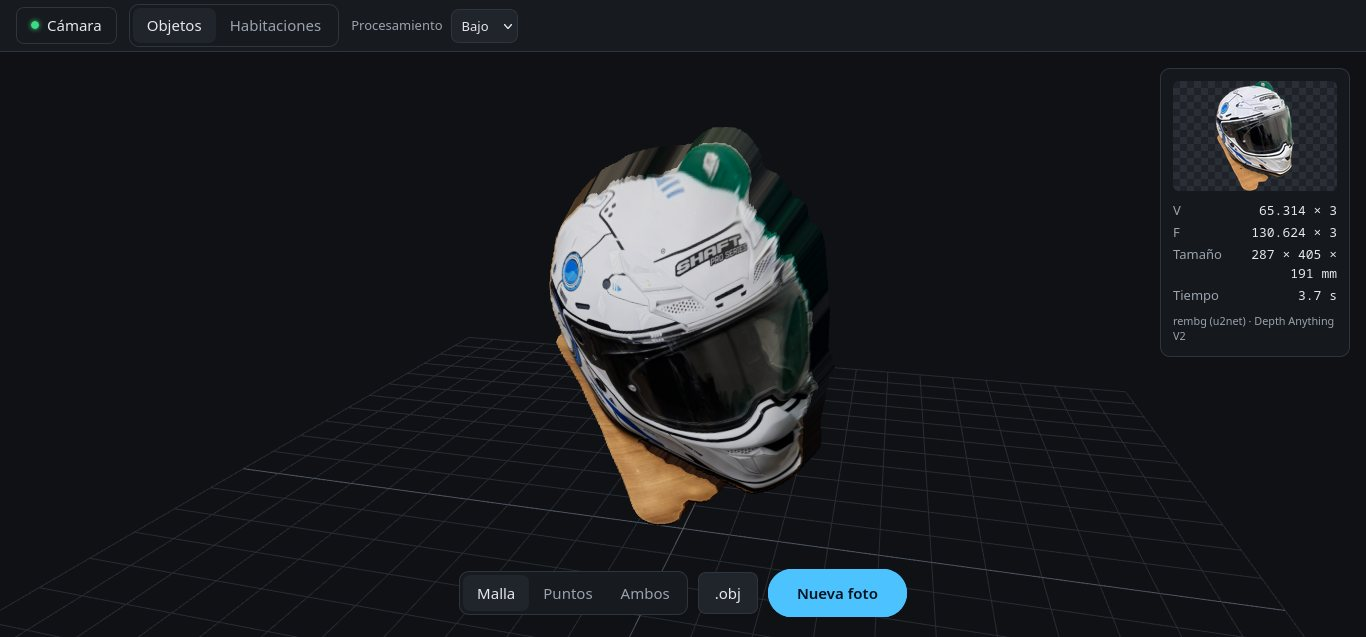
\includegraphics[width=\linewidth]{web_casco_bajo_malla.jpg}
\caption{Pestaña del escáner 3D con el casco en procesamiento bajo: malla con la foto como textura y ficha con el tamaño de $V$ y $F$, las medidas
y el tiempo de cálculo.}
\label{fig:visor-bajo}
\end{figure}

\begin{figure}[htbp]
\centering
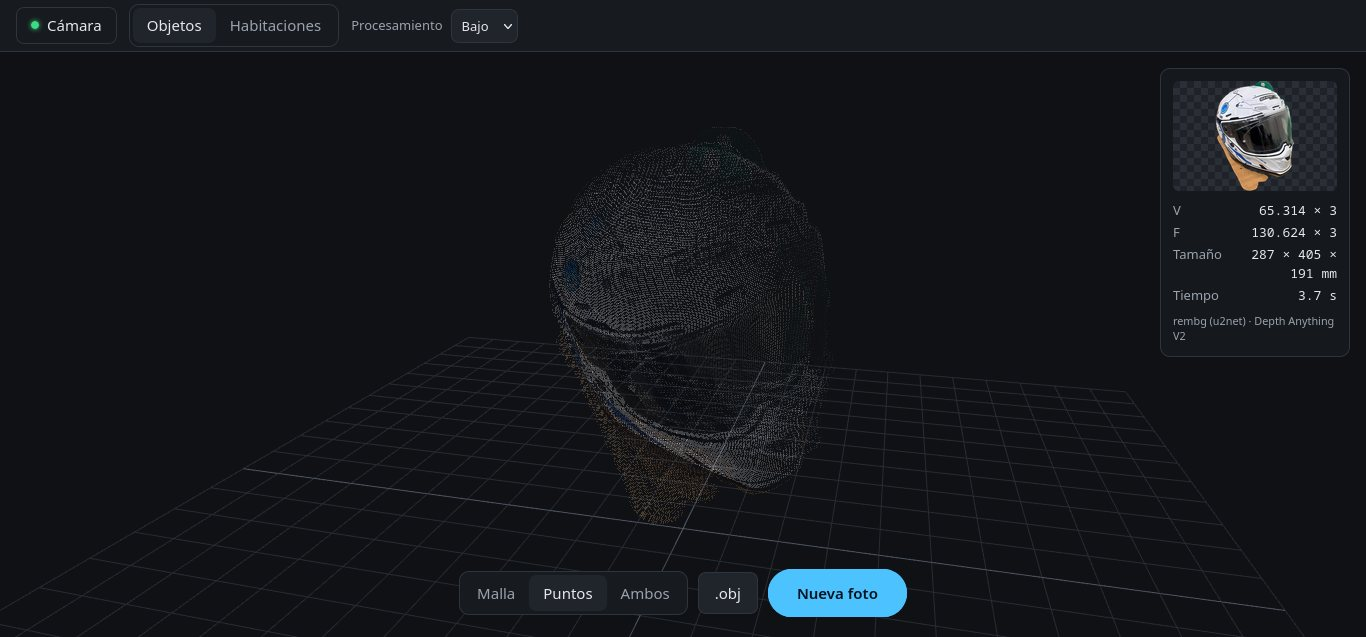
\includegraphics[width=\linewidth]{web_casco_bajo_puntos.jpg}
\caption{El mismo modelo como nube de puntos (la matriz $V$, sin la matriz $F$).}
\label{fig:visor-puntos}
\end{figure}

\begin{figure}[htbp]
\centering
\begin{minipage}{0.48\linewidth}\centering
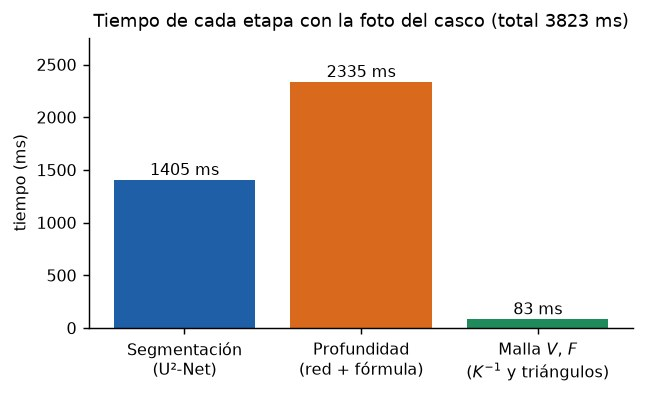
\includegraphics[width=\linewidth]{casco_tiempos_etapas.jpg}
\end{minipage}\hfill
\begin{minipage}{0.48\linewidth}\centering
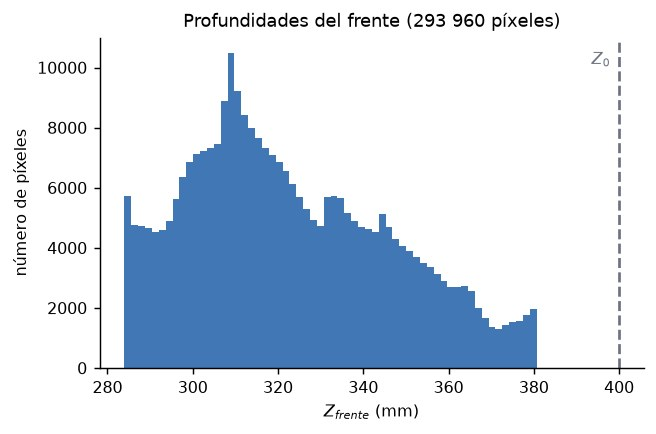
\includegraphics[width=\linewidth]{casco_histograma.jpg}
\end{minipage}
\caption{Izquierda: tiempo de cada etapa para el casco. Derecha: distribución de las profundidades $Z_{\text{frente}}$ de los píxeles del casco
(más cerca de la cámara hacia la izquierda).}
\label{fig:casco-tiempos}
\end{figure}

\begin{figure}[htbp]
\centering
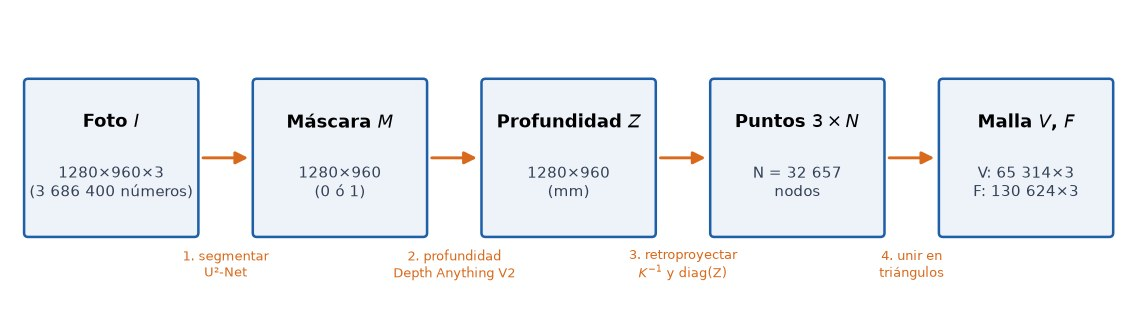
\includegraphics[width=0.8\linewidth]{casco_flujo.jpg}
\caption{Tamaño de cada objeto matemático a lo largo del proceso para el casco: de una matriz de $1280\times960\times3$ números a las matrices
$V$ y $F$.}
\label{fig:casco-flujo}
\end{figure}

\paragraph{Lectura del resultado.} En el visor se reconoce el casco con sus gráficos azules y la visera. Dos defectos son propios del método
con una sola foto: la máscara recorta junto con el casco un pedazo del pupitre sobre el que está apoyado y parte del espaldar verde de la silla (la red los toma como parte del objeto), y
los costados que la cámara no ve quedan estirados, porque la forma se supone redondeada. Con procesamiento alto (cuadro~\ref{tab:alto}) el modelo generativo reconstruye también la parte de atrás y los costados, y el resultado es más completo que el de la extrusión (figura~\ref{fig:visor-alto}); también reproduce, como parte del objeto, el espaldar verde que la máscara dejó pegado al casco.

\begin{figure}[htbp]
\centering
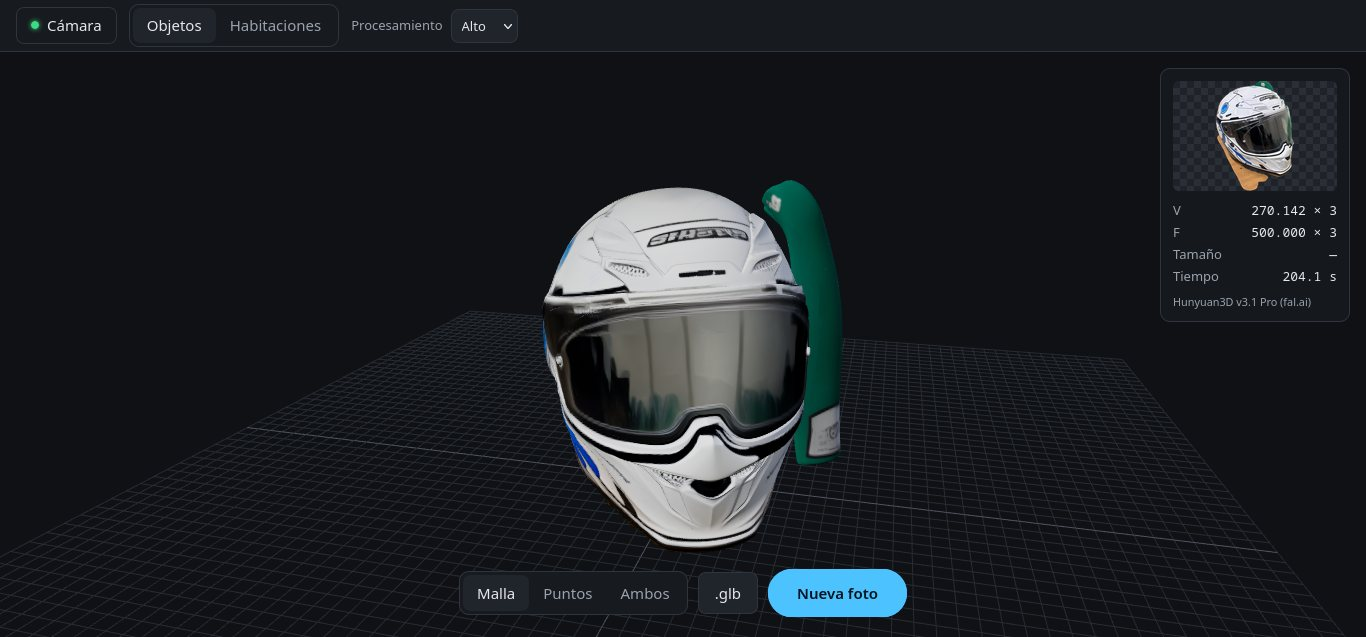
\includegraphics[width=\linewidth]{web_casco_alto.jpg}
\caption{Pestaña del escáner 3D con el casco en procesamiento alto: modelo generativo con textura.}
\label{fig:visor-alto}
\end{figure}
